%\documentclass[openany]{book}
\documentclass[12pt]{article}
\usepackage[utf8]{inputenc}
\usepackage{amssymb} %for fancy L
\usepackage{calrsfs} %for fancy L
\usepackage{cancel}
\usepackage{tabularx}
\usepackage[hyphens]{url}
\usepackage{booktabs}
\usepackage{graphicx}
\usepackage[titletoc,title]{appendix}
\usepackage{subfig}
\DeclareMathAlphabet{\pazocal}{OMS}{zplm}{m}{n} %for fancy L
\usepackage{epsfig, float,array,tabu,longtable,}
\usepackage{hyperref,wrapfig}
\usepackage{enumerate}
\usepackage{graphicx,psfrag}
\usepackage{cite}
\usepackage{sectsty}
\usepackage{epstopdf}
\usepackage{amsmath,esint, setspace, fancyhdr, amsfonts, bookmark, blindtext}
\usepackage[normalem]{ulem}
\usepackage{tikz}
\usepackage{rotating}
\usepackage[americanvoltages,fulldiodes,siunitx]{circuitikz}
\usepackage{stackengine}
\usetikzlibrary{matrix}
\usepackage{multirow}
\usepackage{multicol}
\usetikzlibrary{shapes,backgrounds,patterns}
\usetikzlibrary{mindmap,trees,decorations.markings}
\usetikzlibrary{quotes,angles}
\usepackage{verbatim}
\renewcommand{\baselinestretch}{1}
\setlength{\textheight}{8in}
\setlength{\textwidth}{6.5in}
\setlength{\headheight}{0in}
\setlength{\headsep}{0.25in}
\usepackage{graphicx}
\setlength{\topmargin}{0in}
\setlength{\oddsidemargin}{0in}
\setlength{\evensidemargin}{0in}
\setlength{\parindent}{.3in}
\usepackage{listings}
\usepackage{color} %red, green, blue, yellow, cyan, magenta, black, white
\definecolor{mygreen}{RGB}{28,172,0} % color values Red, Green, Blue
\definecolor{mylilas}{RGB}{170,55,241}
\doublespacing
\begin{document}


\begin{titlepage}

\newcommand{\HRule}{\rule{\linewidth}{0.5mm}} % Defines a new command for the horizontal lines, change thickness here

\center % Center everything on the page
 
%---------------------------------------------------------
%	HEADING SECTIONS
%---------------------------------------------------------

\textsc{\LARGE Colorado School of Mines}\\[1.5cm] % Name of your university/college
\textsc{\Large CSCI 444}\\[0.5cm] % Major heading such as course name
\textsc{\large Advanced Computer Graphics}\\[0.5cm] % Minor heading such as course title

%---------------------------------------------------------
%	TITLE SECTION
%---------------------------------------------------------

\HRule \\[0.6cm]
{ \huge \bfseries Project Proposal}\\[0.4cm] % Title of your document
\HRule \\[1.0cm]
 
%---------------------------------------------------------
%	AUTHOR SECTION
%---------------------------------------------------------

\begin{minipage}{0.4\textwidth}
    \begin{flushleft}
        \emph{Author:}  
        \medskip
        {\textsc{\textbf{Robinson Merillat }}}   % Your name, bold and small caps    
    \end{flushleft}
\end{minipage}
\begin{minipage}{0.45\textwidth}
    \begin{flushright} \large
        \emph{Supervisor:}
        {\textsc{\textbf{Dr. Jeffery Paone }}} % Supervisor's Name
    \end{flushright}
\end{minipage}\\[1cm]

%---------------------------------------------------------
%	DATE SECTION
%---------------------------------------------------------
\begin{center}
{\large \today}
\end{center}
 % Date, change the \today to a set date if you want to be precise

%---------------------------------------------------------
%	LOGO SECTION
%---------------------------------------------------------
%\vfill
\newcommand*{\plogo}{\includegraphics[width=0.25\textwidth]{imgs/mines.png}}

\plogo\\[1cm] % Include a department/university logo - this will require the graphicx package
 
%---------------------------------------------------------

\vfill % Fill the rest of the page with whitespace
\end{titlepage}

\newpage
\tableofcontents
\newpage

% SUMMARY %%%%%%%%%%%%%%%%%%%%%%%%%%%%%%%%%%
\section{Summary}
The world builder is a random terrain generator base upon a random selection of an ecosystem. 
Several different ecosystems could be generated such as mountains, desert, caverns, and islands.
This terrain will be populated with various flora and if time permits, fauna as well (possibly animated, but non-moving). 

\section{Research into the Topic}
One of the largest users of procedurally generated terrain is the Video Game Industry.
A multitude of games impliment procedural terrain techniques such as Minecraft, Spore, Civilization, 
Diablo, and Left 4 Dead just to name a few. These techniques are even used in film such as in the \textit{MASSIVE} 
engine used in Perter Jackson's The Lord of the Rings to generate signifigantly larger combatting armies than 
cast that was at his disposal. Each variation of procedural generation utalizes a different algoritm in order to 
simulate the real world. Several of these algorithms impliment various uses of generated noise such as in the 
simplex noise algorithm while others use various clumping or boring algorithms such in the case of generating 
forests and caves.

\begin{center}
    \includegraphics[width=0.9\textwidth]{imgs/noise.png}
\end{center}

\subsection{Height Mapping}

One of the main basis for procedurally generated terrain is the use of heightmapping. As opposed to procedurally 
generating geometry, heighmapping procedurally generates a black and white texture. When a plane is sent through a 
vertex shader, the y value (vertical) of each vertex is then set to be some scaled value coresponding to the shade 
(0-255) of the texture at that location, thus generating a unique terrain that ultimately saves an imense amount of 
computation time. On top of this, normal mapping techniques are often used along with several other texturing 
techniques to make a realistic looking environment.

\begin{center}
    \begin{minipage}{0.45\textwidth}
        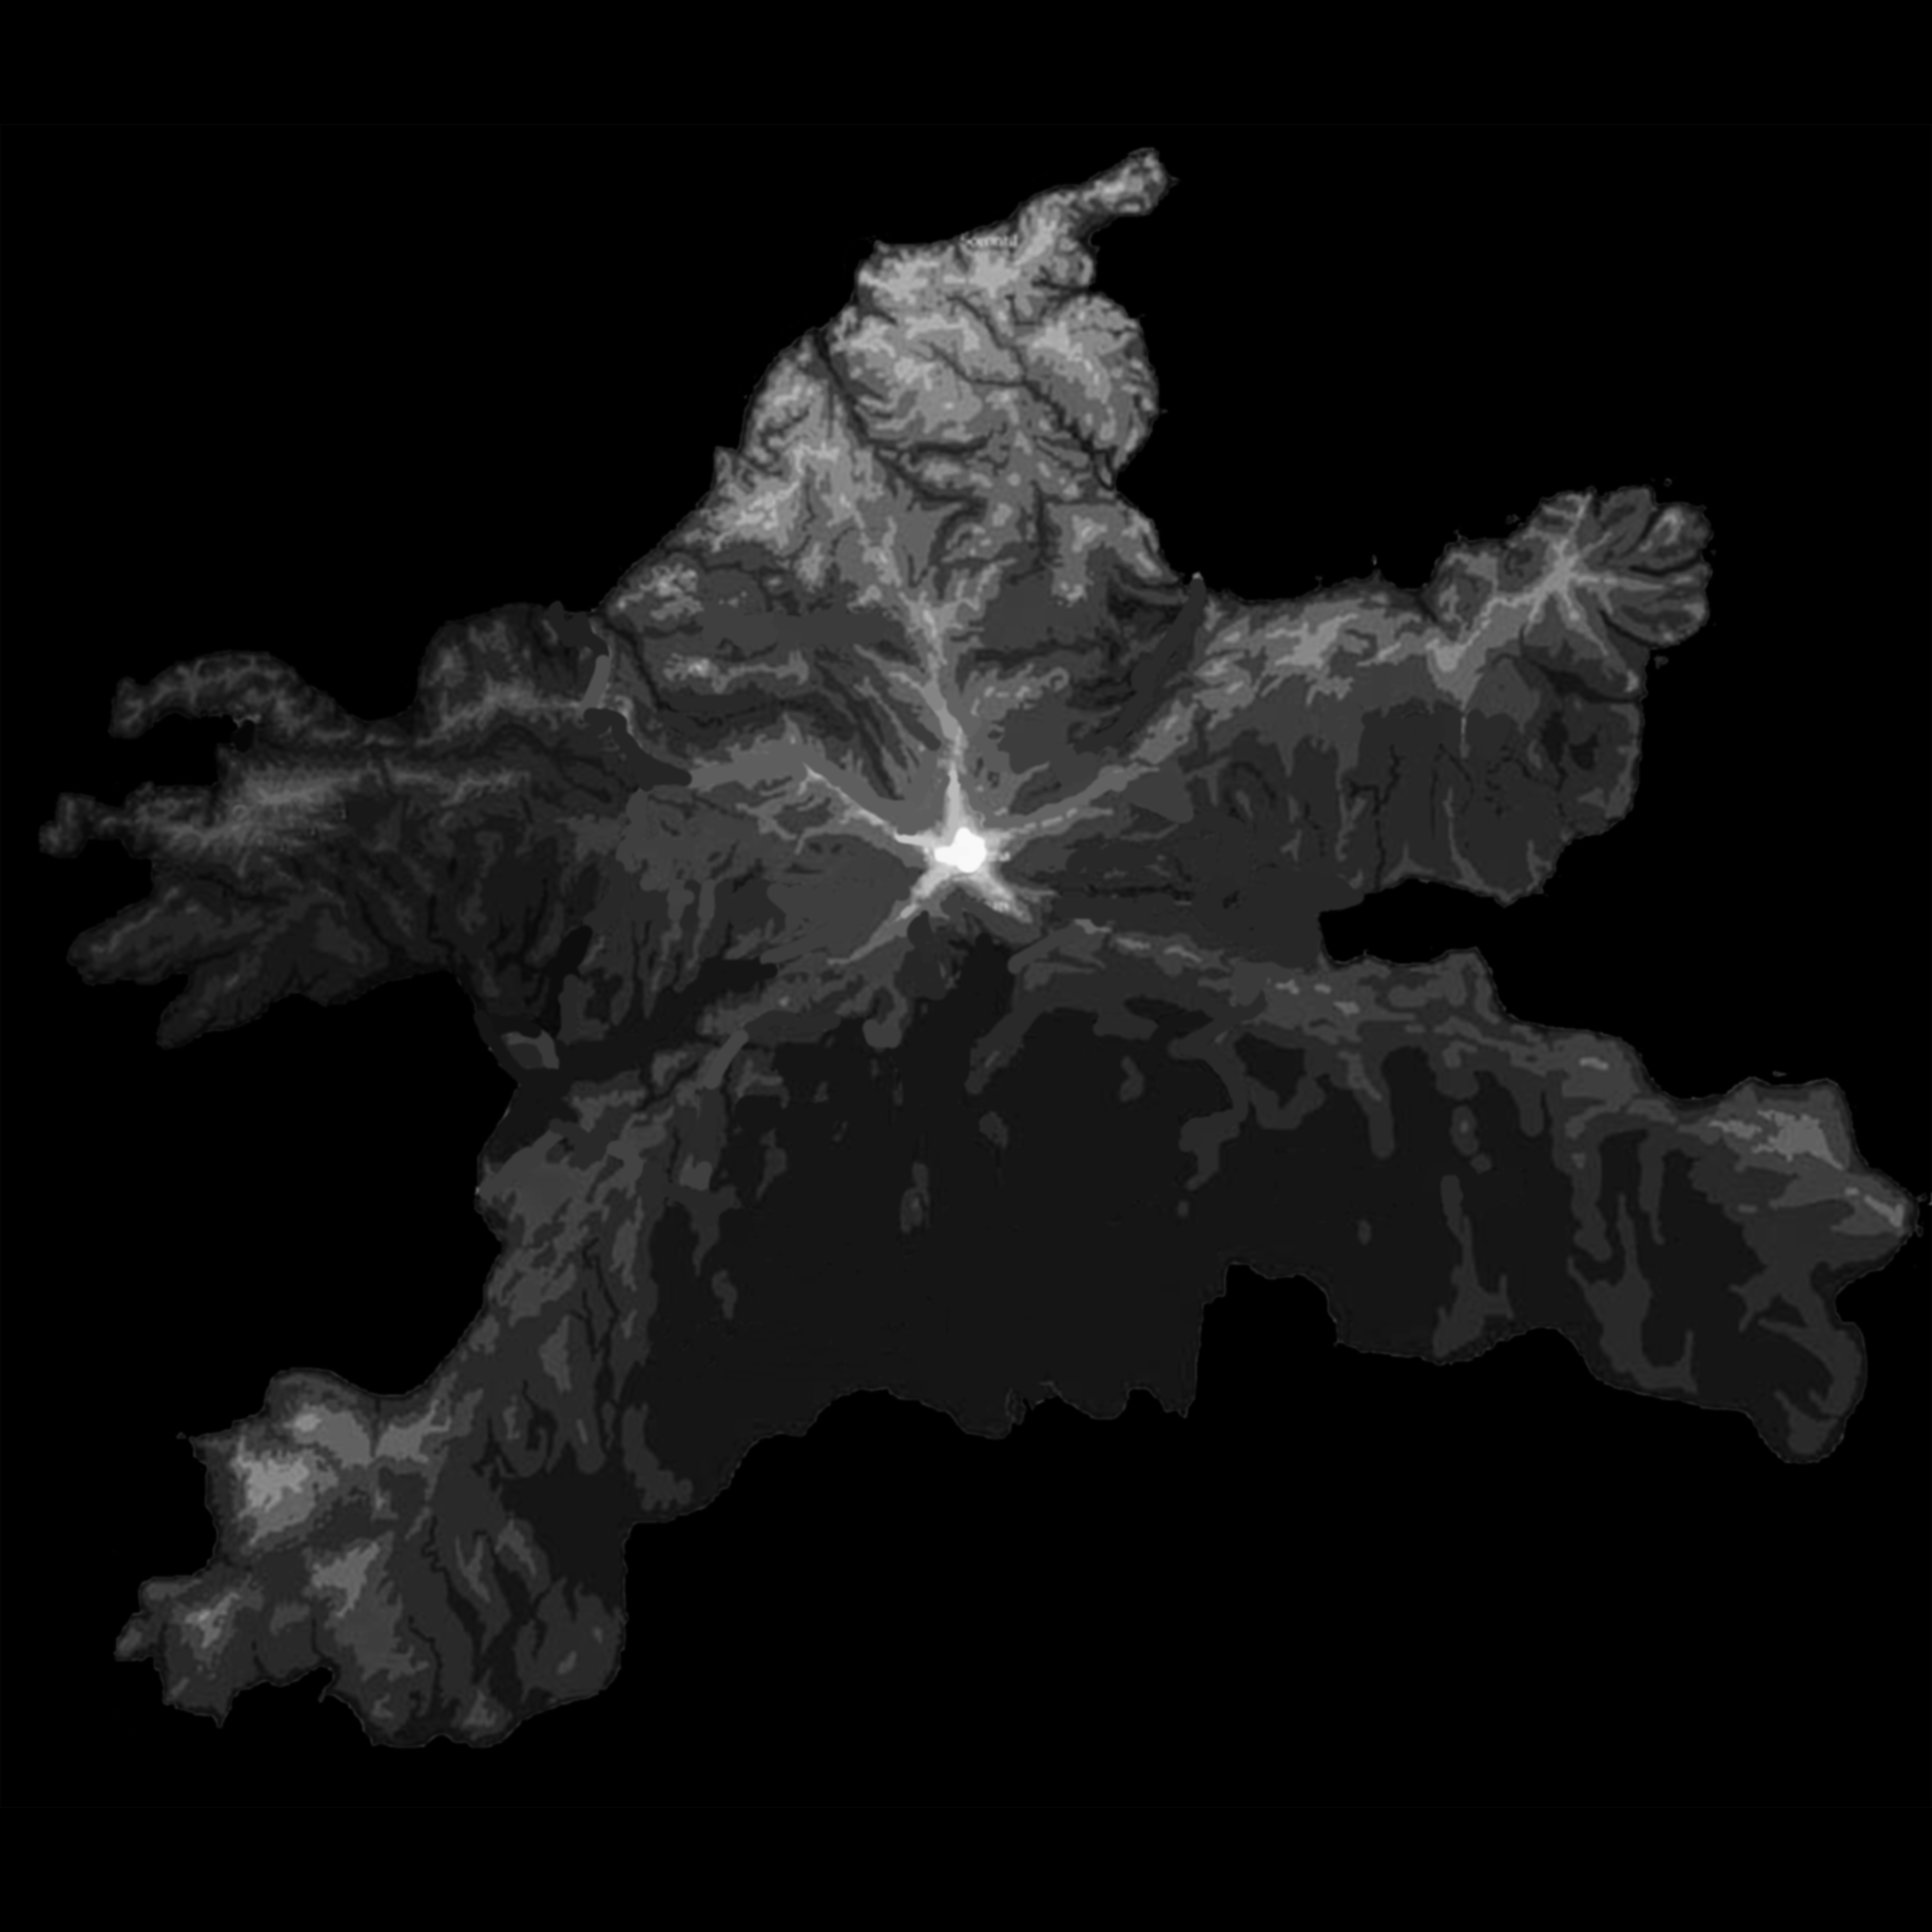
\includegraphics[width=0.75\textwidth]{imgs/EyCkvNy.png}
    \end{minipage}
    \begin{minipage}{0.45\textwidth}
        \includegraphics[width=0.9\textwidth]{imgs/height.jpg}
    \end{minipage}
\end{center}

\subsection{Goals/ Stretch Goals}

Wrapping this back around to this project, the overall goal of this project is to be able to utalize all of these 
graphical techniques to generate procedural interesting and semi-realistic looking terrain of various regions of our,
and enven fantastical worlds. Some stretch goals I would like to look into should I complete the basis of this project 
would be to add models such as trees, rocks, and grasses using grouping algorithms.

\section{Technical Challenges}
    \subsection{Multiple noise/generation algorithms simultaneously}
        The algoritms that are used to generate heightmaps for a mountain or island are not the same as what would 
        generate a tundra or desert. similarly, ice holds a different texture than cracked dry earth. That being said, there
        are many similarities. Exploring those similarities and how I may be able to utalize aspects of each of them to 
        compute the otehrs is a technical challenge that I will surely face.

    \subsection{Minimising Shaders}
        It's easy to get carried away with shaders and start to impliment a new one for every new thing you create,
        however, there is a limit to the number of shaders that can be used. In addition, why recreate a similar shader
        for a new object when you may be able to accomidate it in the one that currently exists. One of the challenges I will face
        is determining when and where it is appropriate to create a new shader.
 
    \subsection{Graphical Techniques}
        Beyond the sheer monstrocity that this project is sure to become, it will be challenging to impliment so many 
        generation techniques simultaneously. I will be using a full range of techniques that I learned throughout the course 
        of the semester and it will chalange me to make something spectacular.\\
        
        Of the techniques learned in this course, I plan on using:
        \begin{itemize} 
            \item UBO's
            \item procedural noise
            \item deferred shading
            \item tesselation shaders to minimize geometry based on proxemity
            \item heightmaps
        \end{itemize}
        
        (note: this is subject to change if I learn something new that I would like to use after beginning this project)

\section{Examples}
\begin{enumerate}
    \item \href{https://threejs.org/examples/webgl_terrain_dynamic.html}{WebGL Procedural Terrain}
    \item \href{http://swordartonline.wikia.com/wiki/Cardinal_System}{Anime Concept of Procedurally Generated Floors/Dungeons/Quests}
    \item \href{https://www.engadget.com/2015/03/04/how-minecraft-worlds-are-made/}{Minecraft world generation}
\end{enumerate}

\end{document}

